\documentclass[a4paper,titlepage,12pt]{scrartcl}	%El modo de documento es para la numeración.

\usepackage{graphicx} %Imágenes
\usepackage[utf8]{inputenc} %Tildes
\usepackage[spanish,es-tabla]{babel} %Español, es-table: llamar tablas en vez de cuadros
\usepackage[breaklinks=true]{hyperref} %Hiperenlaces
\usepackage{amssymb, amsmath, amsbsy} %Símbolos matemáticos
\usepackage{float} %Mover las imágenes usando [H]
\usepackage{eurosym} %Símbolo de euro \euro
\usepackage{listings} %Código
\usepackage{listingsutf8} %Tildes en listings

\numberwithin{figure}{section} %Hace que la primera figura de cada sección X sea X.1
\numberwithin{table}{section} %Hace que la primera tabla de cada sección X sea X.1

\begin{document}
	\lstset{inputencoding=utf8/latin1} %Tildes en listlings
	\begin{titlepage}
		\begin{center}
			\begin{figure}[htb]
				\begin{center}
					
\includegraphics[width=12cm]{./Portada/ugr.png}
				\end{center}
			\end{figure}

			\vspace*{0.8cm}
			\begin{Large}
				\textbf{Grado en Ingeniería Informática.}\\
			\end{Large}
			\begin{Huge}
				\vspace{1.5cm}
				\textbf{Práctica 4.} \\
			\end{Huge}
			\vspace*{0.76cm}
			\rule{100mm}{0.1mm}\\
			\vspace*{0.5cm}
			\begin{large}
				\textbf{Nombre de la asignatura:}\\
				Ingeniería de Servidores.\\
				\vspace*{0.5cm}
				\textbf{Realizado por:}\\
				Néstor Rodríguez Vico \\

				\vspace*{2cm}
				\begin{figure}[htb]
					\begin{center}
						
\includegraphics[width=5cm]{./Portada/etsiit.png}
					\end{center}
				\end{figure}
				\vspace*{-0.6cm}
				ESCUELA TÉCNICA SUPERIOR DE INGENIERÍAS INFORMÁTICA Y DE TELECOMUNICACIÓN.\\
				\rule{20mm}{0.1mm}\\
				\vspace*{0.6cm}
				Granada, \today.
			\end{large}
		\end{center}
	\end{titlepage}
	
	%--------------Indices--------------
	\tableofcontents
	\clearpage
	\listoffigures %Imagenes
	\listoftables %Tablas
	\clearpage
	%----------------------------------
	
	%%%%%%%%%%%%%%%%%%%%%%%%%%%%%%%%%%%%%%%%%%%%%%%%%%%%
	%%%%%%%%%%%%%%%%%%%% Cuestión 1 %%%%%%%%%%%%%%%%%%%%
	%%%%%%%%%%%%%%%%%%%%%%%%%%%%%%%%%%%%%%%%%%%%%%%%%%%%	
	\section[Cuestión 1: Seleccione, instale y ejecute uno, comente los resultados. Atención: no es lo mismo un benchmark que una suite, instale un benchmark.]{Cuestión 1: Seleccione, instale y ejecute uno, comente los resultados. Atención: no es lo mismo un benchmark que una suite, instale un benchmark.}
	
	Esta cuestión la voy a realizar en Ubuntu Server. Lo primero que tengo que hacer es instalar la suite \textit{Phoronoxi} \cite{phoronix}. Para ello ejecutamos \textit{sudo apt-get install phoronix-test-suite}, como podemos ver en la figura \ref{1-1}.
	
	\begin{figure}[H]
		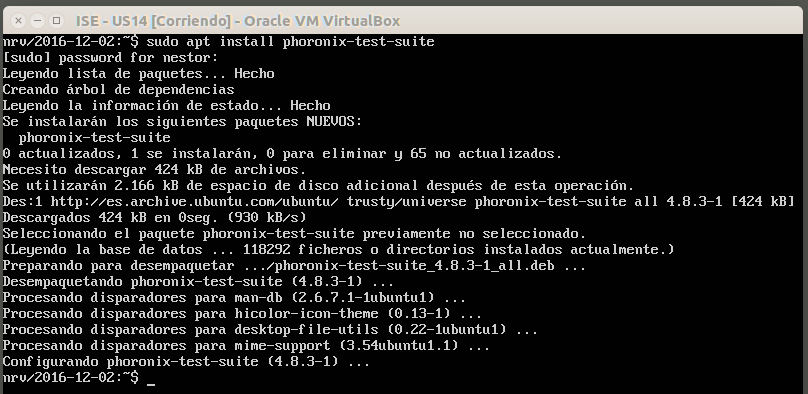
\includegraphics[width=\linewidth]{./Imagenes/1-1.png}
		\vspace{-0.5cm}
		\caption[Instalación de la suite \textit{Phoronix}.]{Instalación de la suite \textit{Phoronix}.}
		\label{1-1}
	\end{figure}
	
	Una vez instalado la suite, listamos los benchmark disponibles ejecutando \textit{phoronix-test-suite list-tests}. Parte de ese listado lo podemos ver en al figura \ref{1-2}. Dado que en la figura \ref{1-3} no podemos ver todos los benchmarks disponibles, recomiendo visitar la página de OpenBenchmarking \cite{openbenchmarking} para poder ver todos los benchmarks disponibles. Una vez hemos elegido el benchmark que queremos ejecutar, \textit{pts/build-apache} en mi caso, lo instalamos con \textit{phoronix-test-suite install pts/build-apache}, como podemos ver en la figura \ref{1-3} y en la figura \ref{1-4}.
	
	\begin{figure}[H]
		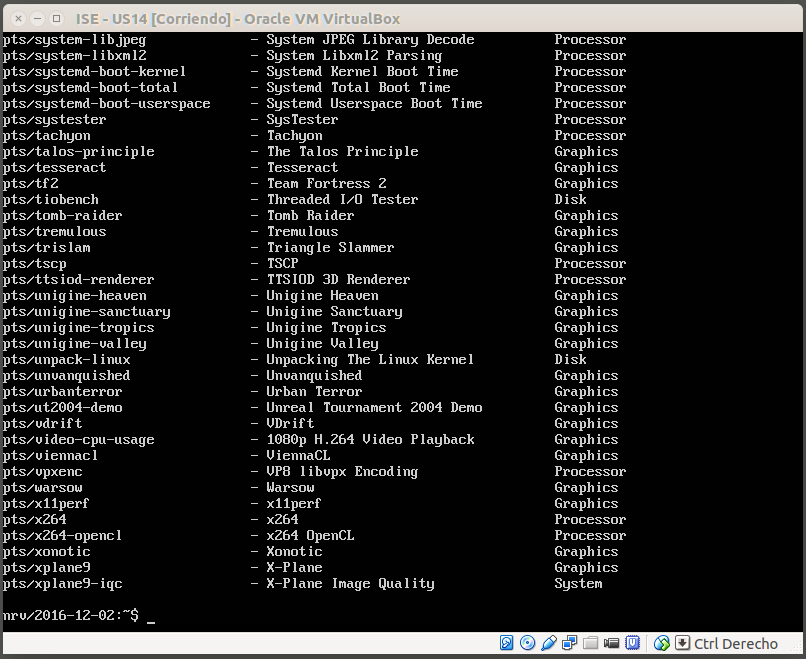
\includegraphics[width=\linewidth]{./Imagenes/1-2.png}
		\vspace{-0.5cm}
		\caption[Benchmarks disponibles.]{Benchmarks disponibles.}
		\label{1-2}
	\end{figure}
	
	\begin{figure}[H]
		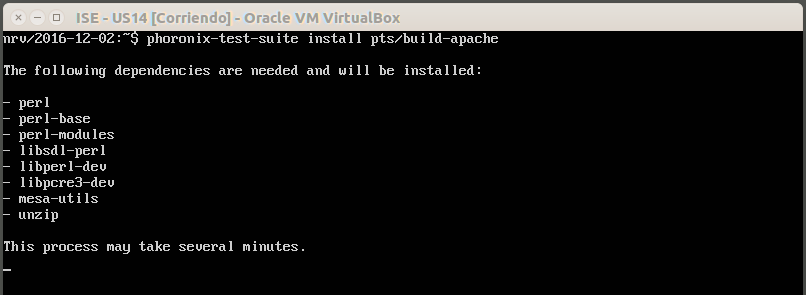
\includegraphics[width=\linewidth]{./Imagenes/1-3.png}
		\vspace{-0.5cm}
		\caption[Instalación del benchmark \textit{pts/build-apache} (1).]{Instalación del benchmark \textit{pts/build-apache} (1).}
		\label{1-3}
	\end{figure}
	
	\begin{figure}[H]
		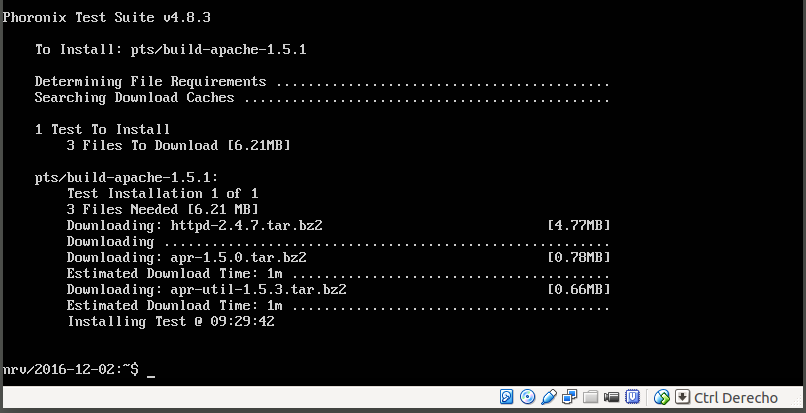
\includegraphics[width=\linewidth]{./Imagenes/1-4.png}
		\vspace{-0.5cm}
		\caption[Instalación del benchmark \textit{pts/build-apache} (2).]{Instalación del benchmark \textit{pts/build-apache} (2).}
		\label{1-4}
	\end{figure}
	
	Una vez instalado, ejecutamos \textit{phoronix-test-suite benchmark pts/build-apache} para iniciar el benchmark. En la figura \ref{1-5} podemos ver los resultados del benchmark. Como podemos ver se han realizado 3 tests, los cuales han tardado 118.5369 segundos, 118.5798 segundos y 118.1869 segundos respectivamente. También podemos ver el instante de tiempo el que se han iniciado los test y el valor medio de todas las ejecuciones, 118.43 segundos en mi caso.
	
	\begin{figure}[H]
		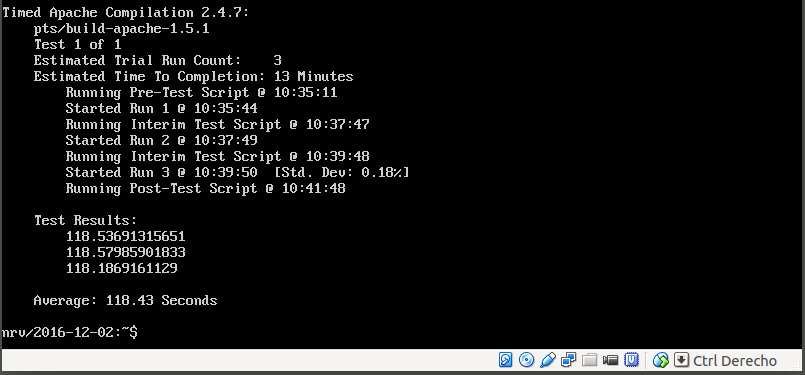
\includegraphics[width=\linewidth]{./Imagenes/1-5.png}
		\vspace{-0.5cm}
		\caption[Resultados del benchmark.]{Resultados del benchmark.}
		\label{1-5}
	\end{figure}
	
	%%%%%%%%%%%%%%%%%%%%%%%%%%%%%%%%%%%%%%%%%%%%%%%%%%%%
	%%%%%%%%%%%%%%%%%%%% Cuestión 2 %%%%%%%%%%%%%%%%%%%%
	%%%%%%%%%%%%%%%%%%%%%%%%%%%%%%%%%%%%%%%%%%%%%%%%%%%%
	\section[Cuestión 2: De los parámetros que le podemos pasar al comando ¿Qué significa -c 5 ? ¿y -n 100? Monitorice la ejecución de ab contra alguna máquina (cualquiera) ¿cuántas “tareas” crea ab en el cliente?]{Cuestión 2: De los parámetros que le podemos pasar al comando ¿Qué significa -c 5 ? ¿y -n 100? Monitorice la ejecución de ab contra alguna máquina (cualquiera) ¿cuántas “tareas” crea ab en el cliente?}
	
	Dicha información la podemos obtener en la documentación de Apache \cite{ab-apache}. El argumento \textit{-c 5} indica la concurrencia, es decir, el número de peticiones que se van a realizar de manera simultánea. El argumento \textit{-n 100} indica el número de solicitudes que se van a realizar durante el benchmark. \\
	
	Voy a ejecutar \textit{ab} contra Ubuntu Server desde mi máquina anfitriona, así que he tenido que instalar \textit{ab} ejecutando \textit{sudo apt install apache2-utils}. Para ello ejecutamos la orden \textit{ab -c 5 -n 100 DireccionIPServidor}. La dirección IP de mi servidor, como podemos ver en la figura \ref{2-1}, es \textit{192.168.56.103} (máquina conectadas en modo \textit{host-only}), así que ejecutamos \textit{ab -c 5 -n 100 http://192.168.56.103}, como podemos ver en la figura \ref{2-1}. Para ver cuantas tareas se han creado en el cliente, ejecutamos \textit{ps -A | grep ab}. Como podemos ver en la figura \ref{2-1} se ha creado sólo una tarea. En la figura \ref{2-2} podemos ver el resultado completo de la monitorización. Podemos ver desde información básica del servidor hasta el número de bytes transferidos o el tiempo de media empleado en los tests.
	
	\begin{figure}[H]
		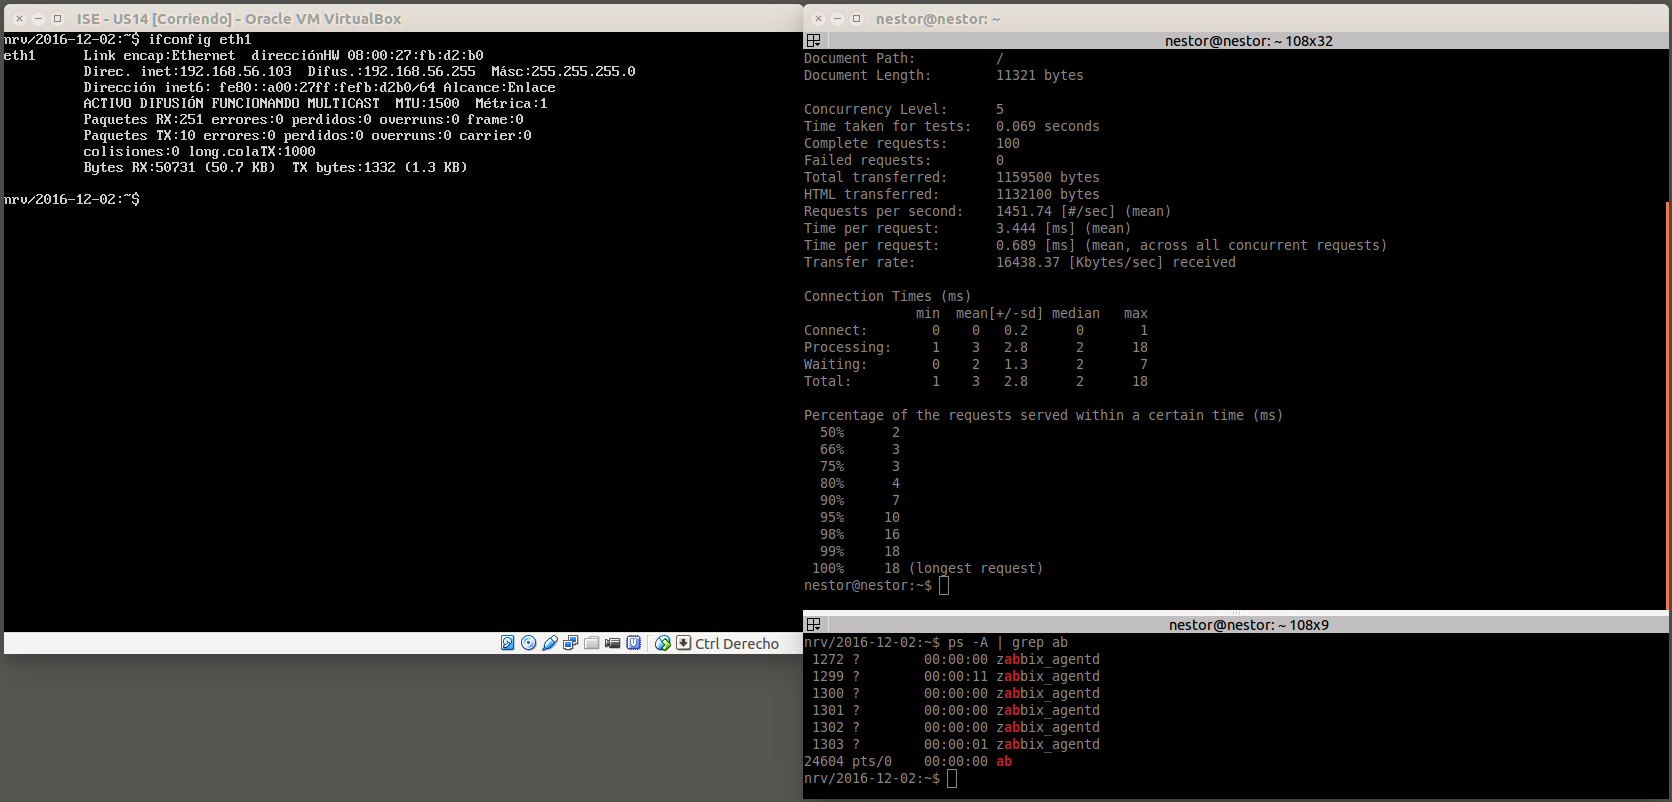
\includegraphics[width=\linewidth]{./Imagenes/2-1.png}
		\vspace{-0.5cm}
		\caption[Resultado parcial de la monitorización y número de tareas creadas.]{Resultado parcial de la monitorización y número de tareas creadas.}
		\label{2-1}
	\end{figure}
		
	\begin{figure}[H]
		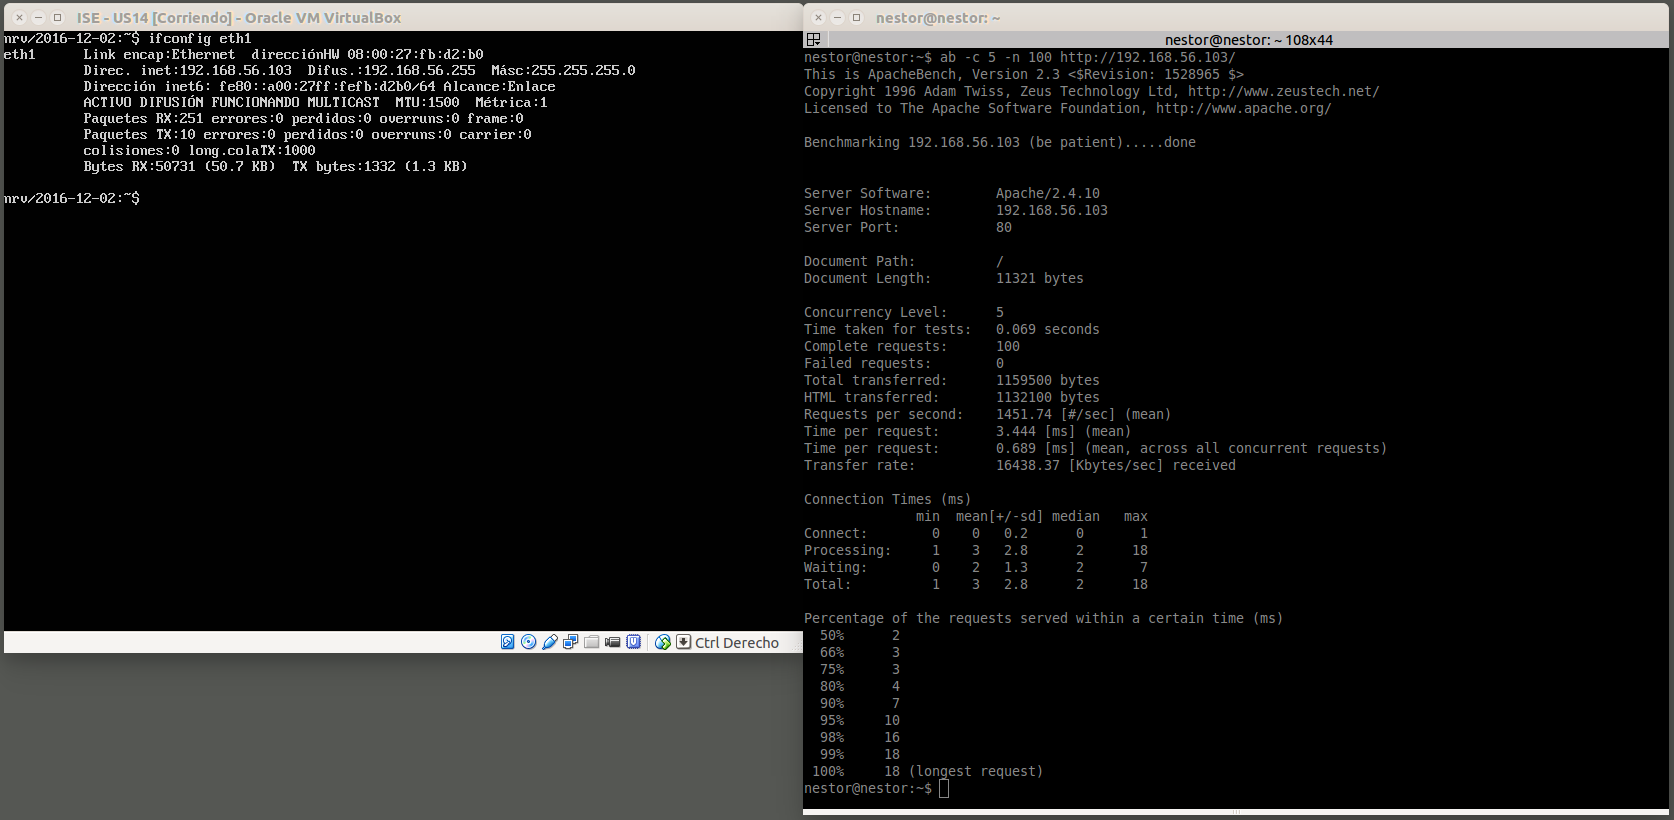
\includegraphics[width=\linewidth]{./Imagenes/2-2.png}
		\vspace{-0.5cm}
		\caption[Resultado completo de la monitorización.]{Resultado completo de la monitorización.}
		\label{2-2}
	\end{figure}
	
	%%%%%%%%%%%%%%%%%%%%%%%%%%%%%%%%%%%%%%%%%%%%%%%%%%%%
	%%%%%%%%%%%%%%%%%%%% Cuestión 3 %%%%%%%%%%%%%%%%%%%%
	%%%%%%%%%%%%%%%%%%%%%%%%%%%%%%%%%%%%%%%%%%%%%%%%%%%%
	\section[Cuestión 3: Ejecute ab contra a las tres máquinas virtuales (desde el SO anfitrión a las máquina virtuales de la red local) una a una (arrancadas por separado).¿Cuál es la que proporciona mejores resultados? Muestre y coméntelos. (Use como máquina de referencia Ubuntu Server para la comparativa).]{Cuestión 3: Ejecute ab contra a las tres máquinas virtuales (desde el SO anfitrión a las máquina virtuales de la red local) una a una (arrancadas por separado).¿Cuál es la que proporciona mejores resultados? Muestre y coméntelos. (Use como máquina de referencia Ubuntu Server para la comparativa).}
	
	Para monitorizar en las mismas condiciones voy a ejecutar el mismo comando desde mi máquina anfitriona (máquinas conectadas en modo \textit{host-only}) y contra la misma página web \footnote{La página web usada se encuentra dentro de la carpeta \textit{Archivos auxiliares} bajo el nombre \textit{``practica4.html''}.}. Dicho archivo lo he ubicado en el directorio \textit{/var/www/} en el caso de Ubuntu Server y CentOS y en el directorio \textit{C:\textbackslash inetpug\textbackslash wwwroot} en el caso de Windows Server. El comando es el mismo que el usado en la cuestión anterior, \textit{ab -c 5 -n 100 DireccionIPServidor}. El resultado de la monitorización en Ubuntu Server lo podemos ver en la figura \ref{3-UbuntuServer}, el resultado de CentOS lo podemos ver en la figura \ref{3-CentOS} y el resultado de Windows Server lo podemos ver en la figura \ref{3-WindowsServer}.
	
	\begin{figure}[H]
		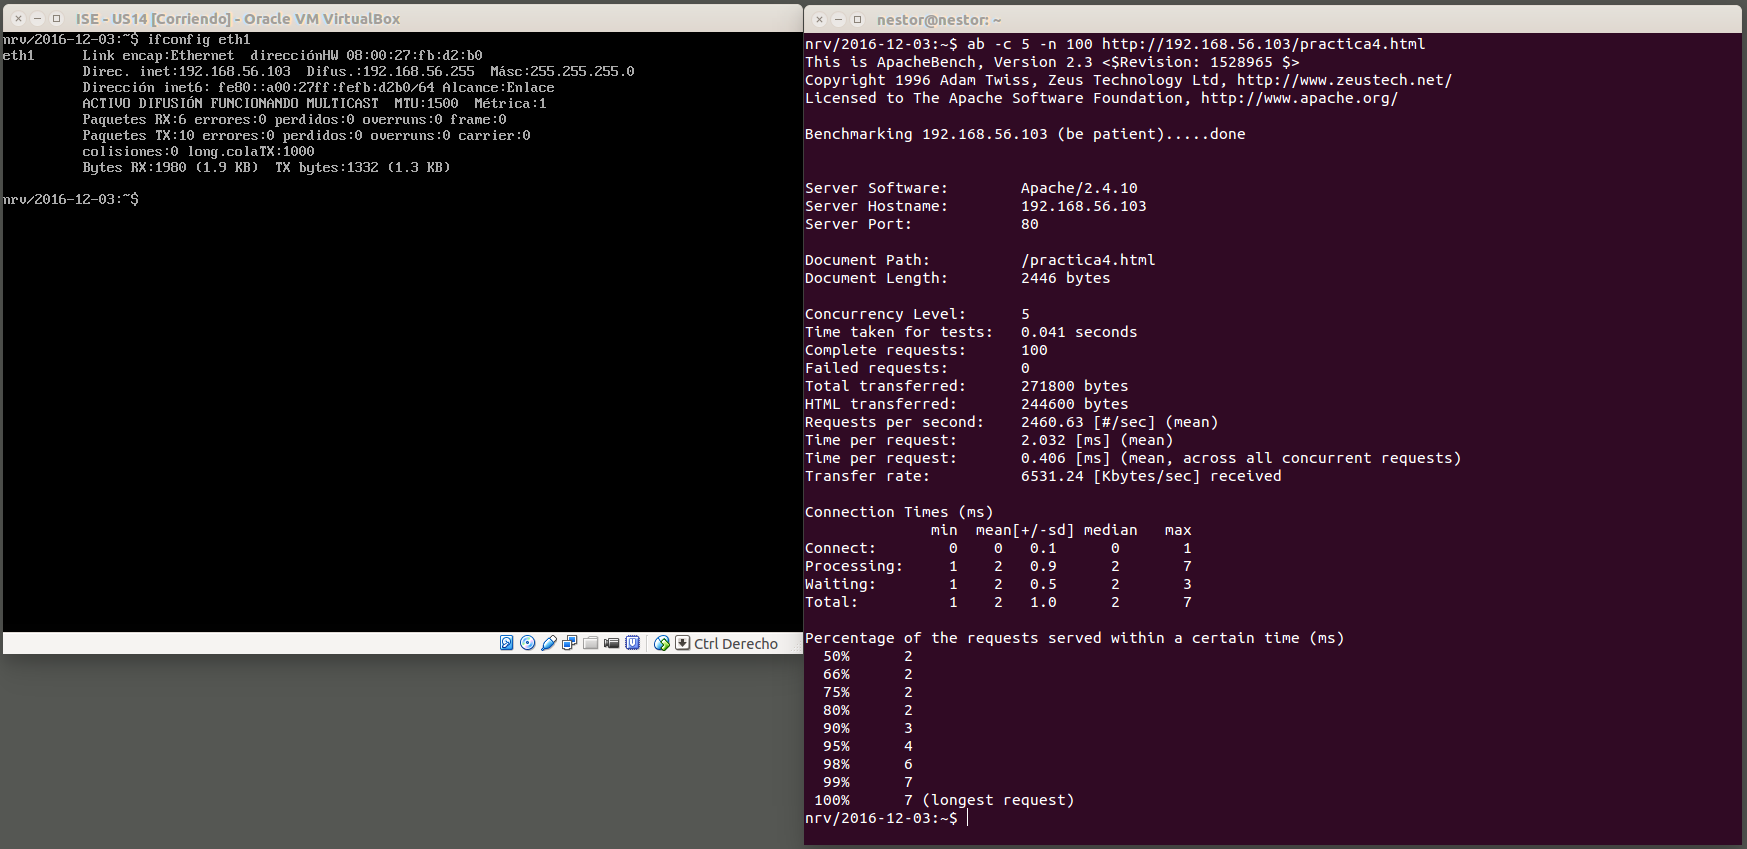
\includegraphics[width=\linewidth]{./Imagenes/3-UbuntuServer.png}
		\vspace{-0.5cm}
		\caption[Resultado de la monitorización en Ubuntu Server.]{Resultado de la monitorización en Ubuntu Server.}
		\label{3-UbuntuServer}
	\end{figure}
	
	\begin{figure}[H]
		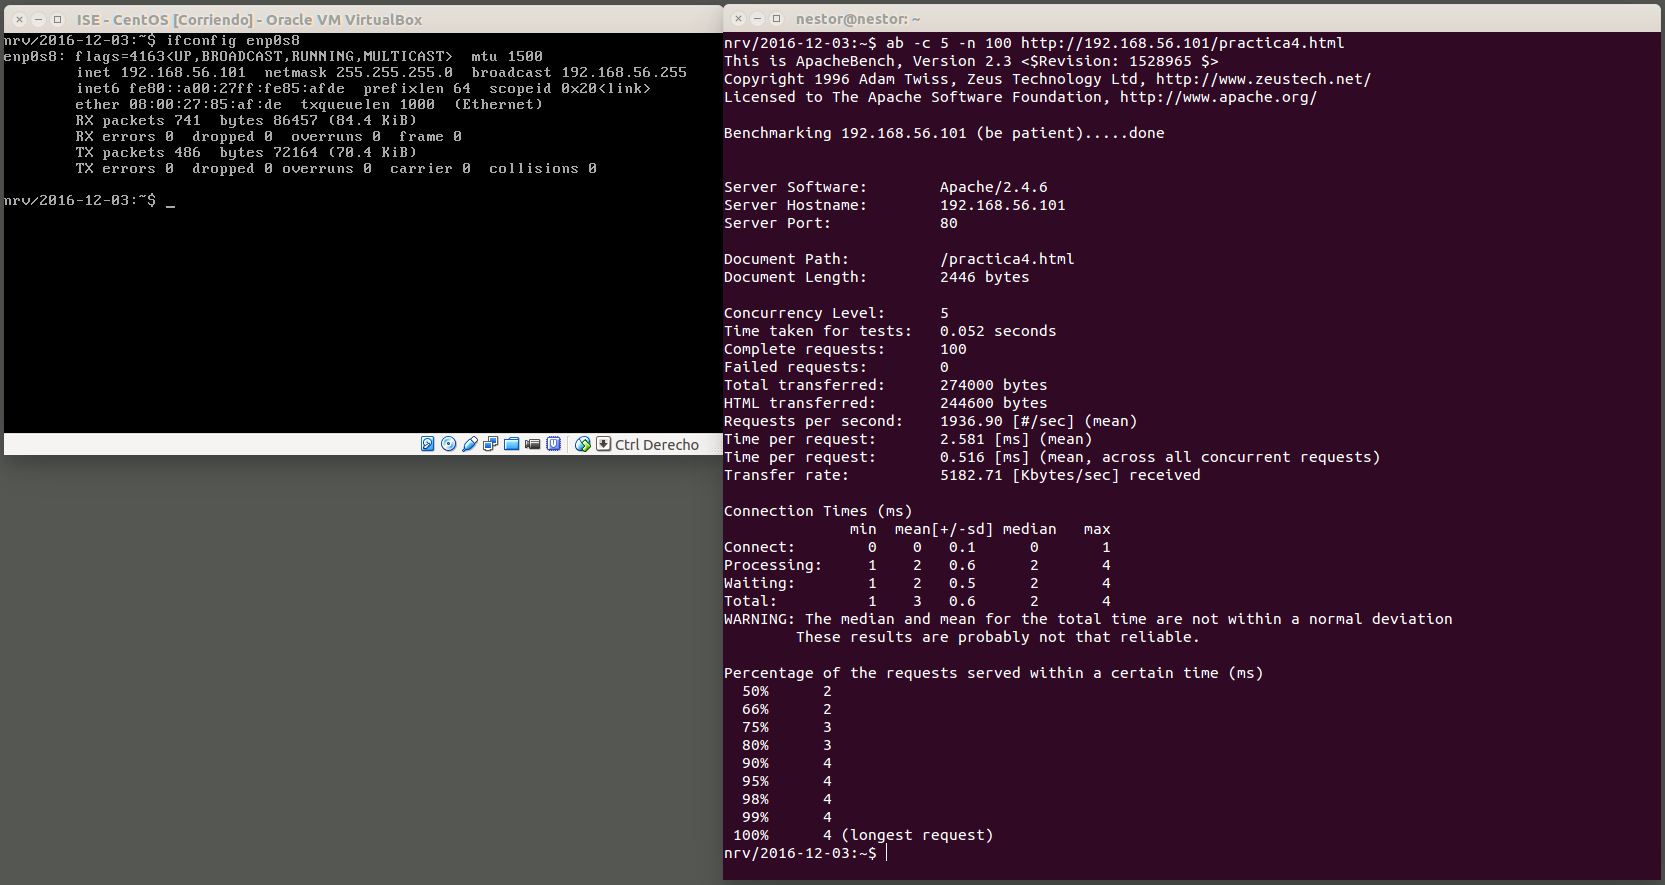
\includegraphics[width=\linewidth]{./Imagenes/3-CentOS.png}
		\vspace{-0.5cm}
		\caption[Resultado de la monitorización en CentOS.]{Resultado de la monitorización en CentOS.}
		\label{3-CentOS}
	\end{figure}
	
	\begin{figure}[H]
		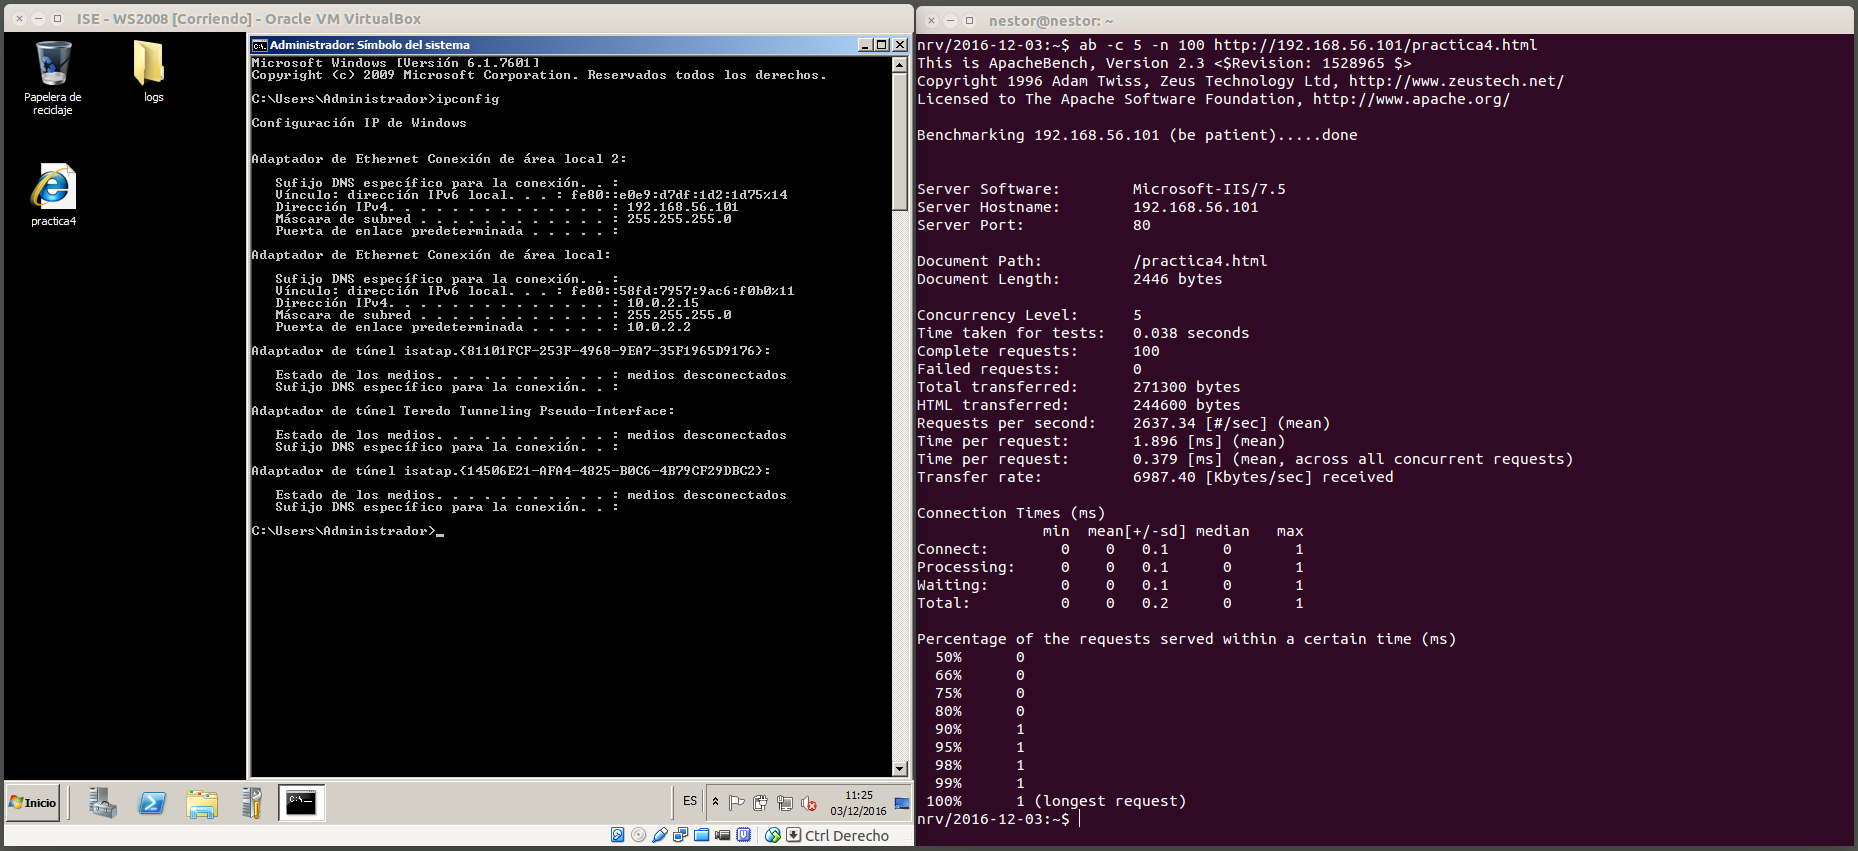
\includegraphics[width=\linewidth]{./Imagenes/3-WindowsServer.png}
		\vspace{-0.5cm}
		\caption[Resultado de la monitorización en Windows Server.]{Resultado de la monitorización en Windows Server.}
		\label{3-WindowsServer}
	\end{figure}
	
	Para poder comparar mejor los resultados, vamos a extraer los datos más relevantes en la tabla \ref{comparacion-apache}:
	
	\begin{table}[H]
		\centering
		\begin{tabular}{|l|c|c|c|c|c|c|}
		\hline
		& \begin{tabular}[c]{@{}c@{}}Tiempo\\ total (s)\end{tabular} & \begin{tabular}[c]{@{}c@{}}Promedio de \\ solicitudes\\ procesadas \\ por segundo\end{tabular} & \begin{tabular}[c]{@{}c@{}}Tiempo \\ medio por \\ solicitud (ms)\end{tabular} & \begin{tabular}[c]{@{}c@{}}Bytes \\ transmitidos\end{tabular} & \begin{tabular}[c]{@{}c@{}}Velocidad de \\ transferencia \\ (KB/s)\end{tabular} \\ \hline
		Ubuntu Server  & 0.041 & 2460.63 & 2.032 & 271800 & 6531.24 \\ \hline
		CentOS         & 0.052 & 1936.90 & 2.581 & 274000 & 5182.71 \\ \hline
		Windows Server & 0.038 & 2637.34 & 1.896 & 271400 & 6987.40 \\ \hline
		\end{tabular}
		\caption{Comparación de los tres sistemas operativos.}
		\label{comparacion-apache}
	\end{table}
	
	Tras observar la tabla, podemos decir que el que mejor resultados ofrece ha sido Windows Server, pero esto no quiere decir que siempre sea mejor, ya que el datos obtenidos pueden variar entre distintas monitorizaciones. También cabe destacar que el número de bytes transmitidos es diferente, a pesar de transmitir la misma página en los tres sistemas operativos.
	
	%%%%%%%%%%%%%%%%%%%%%%%%%%%%%%%%%%%%%%%%%%%%%%%%%%%%
	%%%%%%%%%%%%%%%%%%%% Cuestión 4 %%%%%%%%%%%%%%%%%%%%
	%%%%%%%%%%%%%%%%%%%%%%%%%%%%%%%%%%%%%%%%%%%%%%%%%%%%
	\section[Cuestión 4: Instale y siga el tutorial en http://jmeter.apache.org/usermanual/build-web-test-plan.html realizando capturas de pantalla y comentándolas. En vez de usar la web de jmeter, haga el experimento usando sus máquinas virtuales ¿coincide con los resultados de ab?]{Cuestión 4: Instale y siga el tutorial en http://jmeter.apache.org/usermanual/build-web-test-plan.html realizando capturas de pantalla y comentándolas. En vez de usar la web de jmeter, haga el experimento usando sus máquinas virtuales ¿coincide con	los resultados de ab?}
	
	Voy a monitorizar Ubuntu Server desde mi máquina anfitriona (máquinas conectadas en modo \textit{host-only}). Para ello, instalamos \textit{JMeter} en mi portátil ejecutando \textit{sudo apt install jmeter}. Una vez instalado, lo lanzamos ejecutando \textit{jmeter}. Como bien nos indica el enunciado, voy a seguir la información de \textit{JMeter} \cite{jmeter} para realizar este ejercicio. Los pasos a seguir son los siguientes:
	\begin{enumerate}
		\item Añadimos un grupo de hilos. Un grupo de hilos indica a \textit{JMeter} cuantos usuarios queremos simulas, cuántas peticiones van a mandar y con que frecuencia serán mandadas. Para añadir el grupo de hilos, le damos click derecho a \textit{Plan de Prueba}, luego le damos a \textit{Añadir}, a continuación elegimos \textit{Hilos (Usuarios)} y por último elegimos \textit{Grupo de hilos}.
		\item A continuación configuramos dicho grupo. Los parámetros que he modificado son los que podemos ver a continuación y se ve pueden ver en la figura \ref{4-1}.
		\begin{itemize}
			\item \textbf{Nombre:} Este parámetro es más que nada por estética. En mi caso lo he cambiado a \textit{Usuarios}.
			\item \textbf{Número de Hilos:} En mi caso, voy a simular 30 usuarios.
			\item \textbf{Periodo de subida (en segundos):} En mi caso, lo he dejado a 1, que es el valor por defecto. Este parámetro representa el retraso que se produce entre la creación de dos usuarios.
			\item \textbf{Contador del bucle Count:} Indica cuantas veces \textit{JMeter} debe repetir el test. En mi caso le he indicado que repita el test 20 veces.
		\end{itemize}
		\item Una vez creados los usuarios, vamos a definir las tareas que van a realizar. Para ello seleccionamos \textit{Usuarios}, el grupo que hemos creado en los pasos anteriores, le damos click derecho y elegimos \textit{Añadir}, luego elegimos \textit{Elemento de Configuración} y finalmente \textit{Valores por Defecto para Petición HTTP}. A continuación le indicamos la dirección IP de nuestro servidor, \textit{192.168.56.103} (máquinas conectadas en modo \textit{host-only}). El resto de parámetros los he dejado por defecto, tal y como podemos ver en la figura \ref{4-2}.
		\item Añadimos un gestor de cookies. Para ello seleccionamos \textit{Usuarios}, el grupo que hemos creado en los pasos anteriores, le damos click derecho y elegimos \textit{Añadir}, luego elegimos \textit{Elemento de Configuración} y finalmente \textit{Gestor de Cookies HTTP}.
		\item A continuación añadimos las peticiones HTTP. Para ello seleccionamos \textit{Usuarios}, el grupo que hemos creado en los pasos anteriores, le damos click derecho y elegimos \textit{Añadir}, luego elegimos \textit{Muestreador} y finalmente \textit{Petición HTTP}. Dentro de la petición, indicamos la ruta del archivo HTML, en mi caso he elegido la raíz de mi servidor, \textit{/}, tal y como podemos ver en la figura \ref{4-3}.
		\item Finalmente, añadimos un \textit{Listener} para ver y almacenar los resultados. Para ello seleccionamos \textit{Usuarios}, el grupo que hemos creado en los pasos anteriores, le damos click derecho y elegimos \textit{Añadir}, luego elegimos \textit{Receptor} y finalmente \textit{Gráfico de Resultados}.
		\item A continuación, guardamos nuestro plan de pruebas. Finalmente, lo ejecutamos pulsando el botón \textit{play} verde en el programa.
	\end{enumerate}
	
	\begin{figure}[H]
		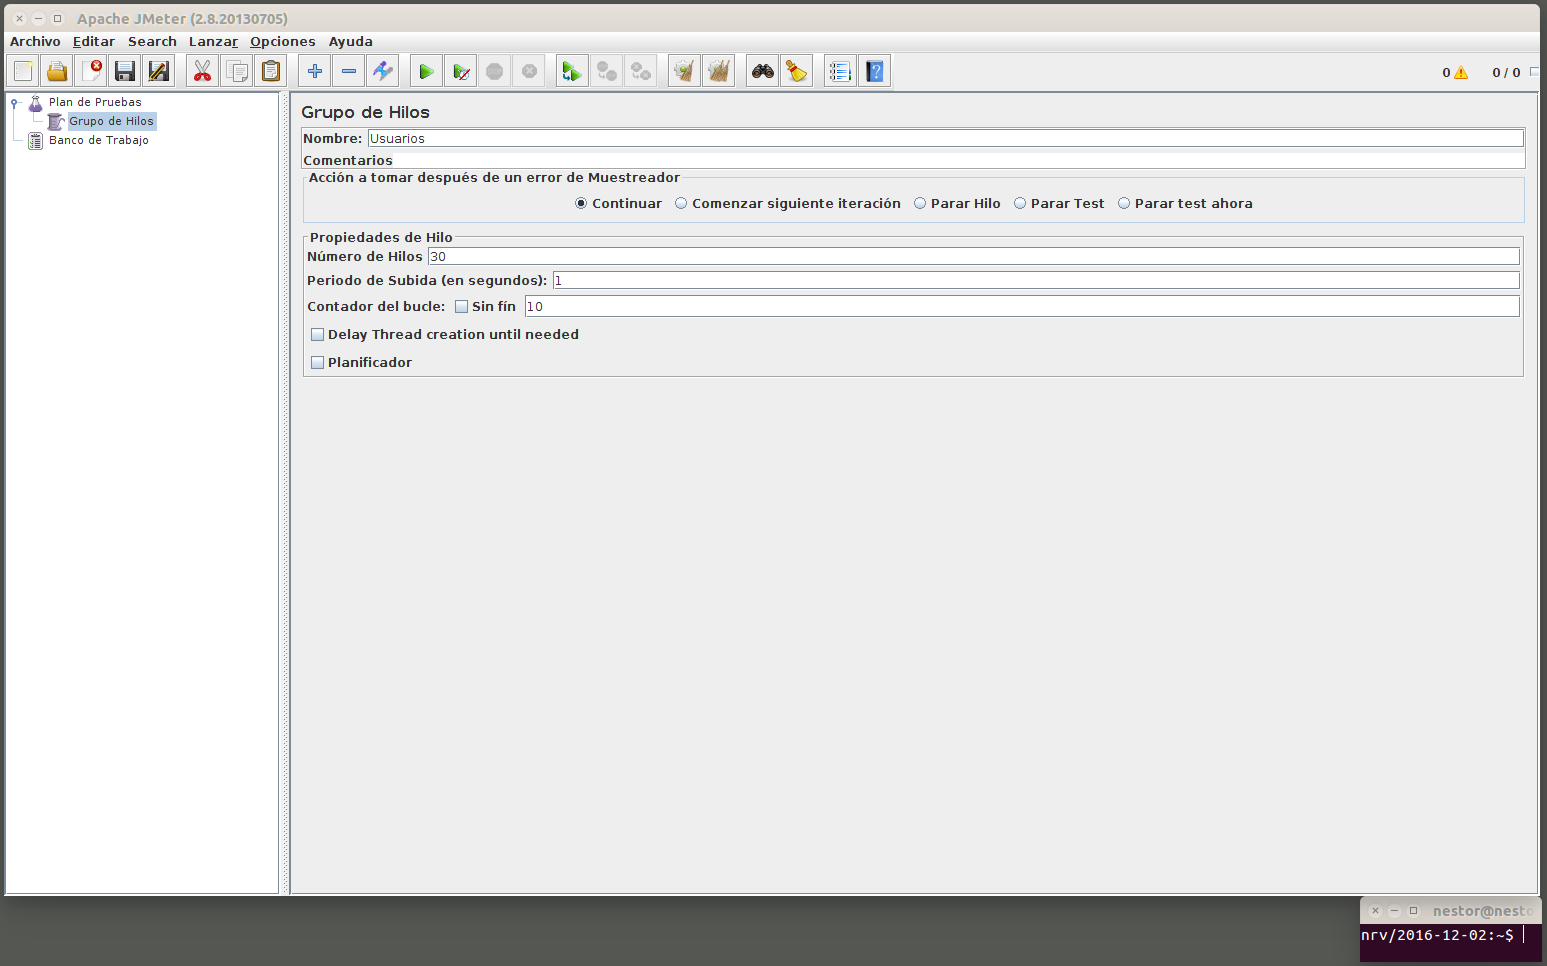
\includegraphics[width=\linewidth]{./Imagenes/4-1.png}
		\vspace{-0.5cm}
		\caption[Creación del grupo de hilos.]{Creación del grupo de hilos.}
		\label{4-1}
	\end{figure}
	
	\begin{figure}[H]
		\centering
		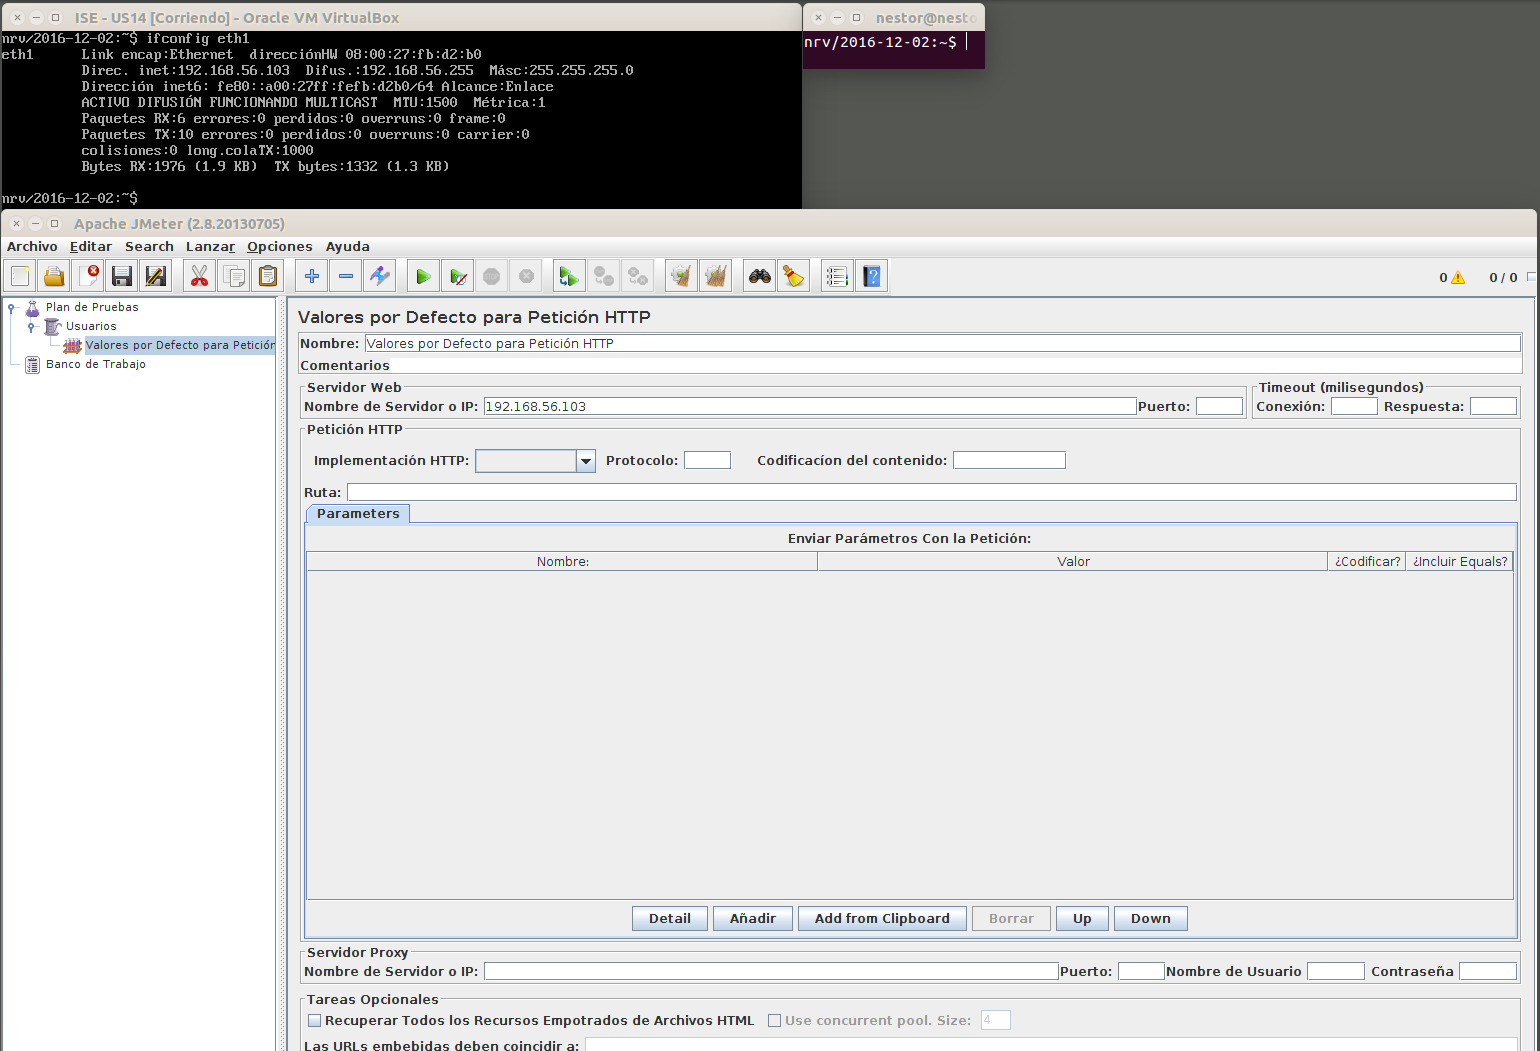
\includegraphics[scale=0.26]{./Imagenes/4-2.png}
		\caption[Configuración de la tarea a realizar por los usuarios.]{Configuración de la tarea a realizar por los usuarios.}
		\label{4-2}
	\end{figure}
	
	\begin{figure}[H]
		\centering
		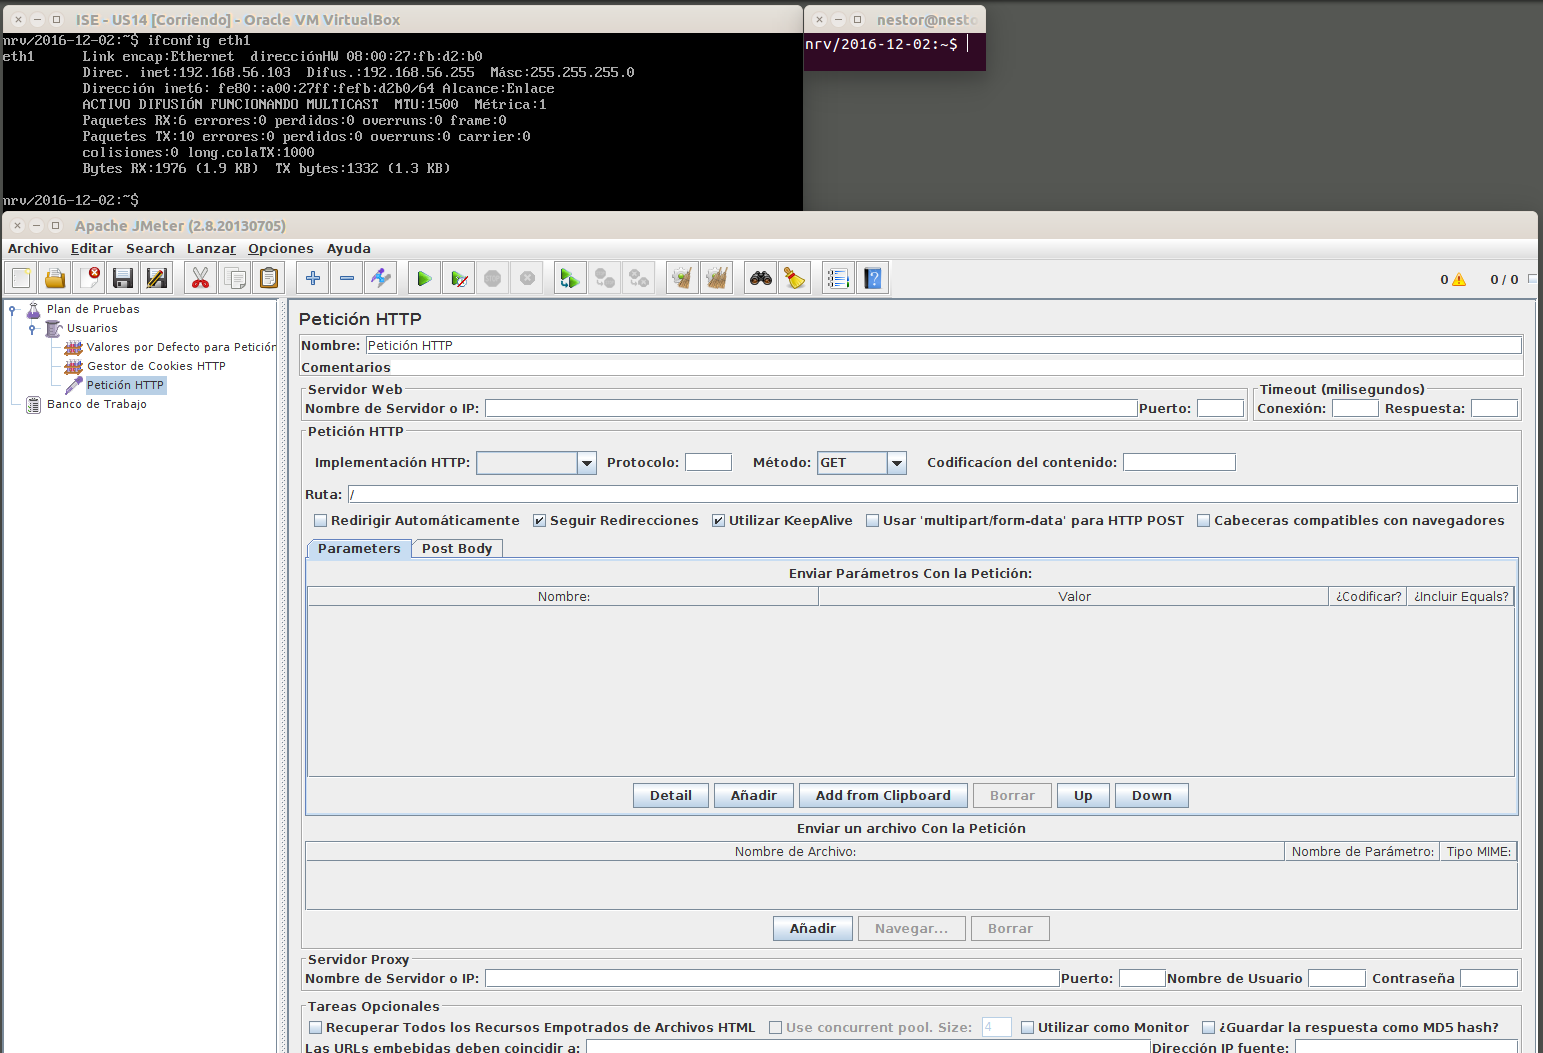
\includegraphics[scale=0.26]{./Imagenes/4-3.png}
		\caption[Configuración de la petición HTTP.]{Configuración de la petición HTTP.}
		\label{4-3}
	\end{figure}
	
	Una ves ejecutado, el resultado lo podemos ver en la figura \ref{4-resultado}. En dicha figura podemos una representación gráfica de los datos recogidos. Los resultados son distintos a los proporcionados por \textit{ab}. Desde mi punto de vista, me gusta más como \textit{ab} representa los datos, ya que veo la información de manera más clara.
	
	\begin{figure}[H]
		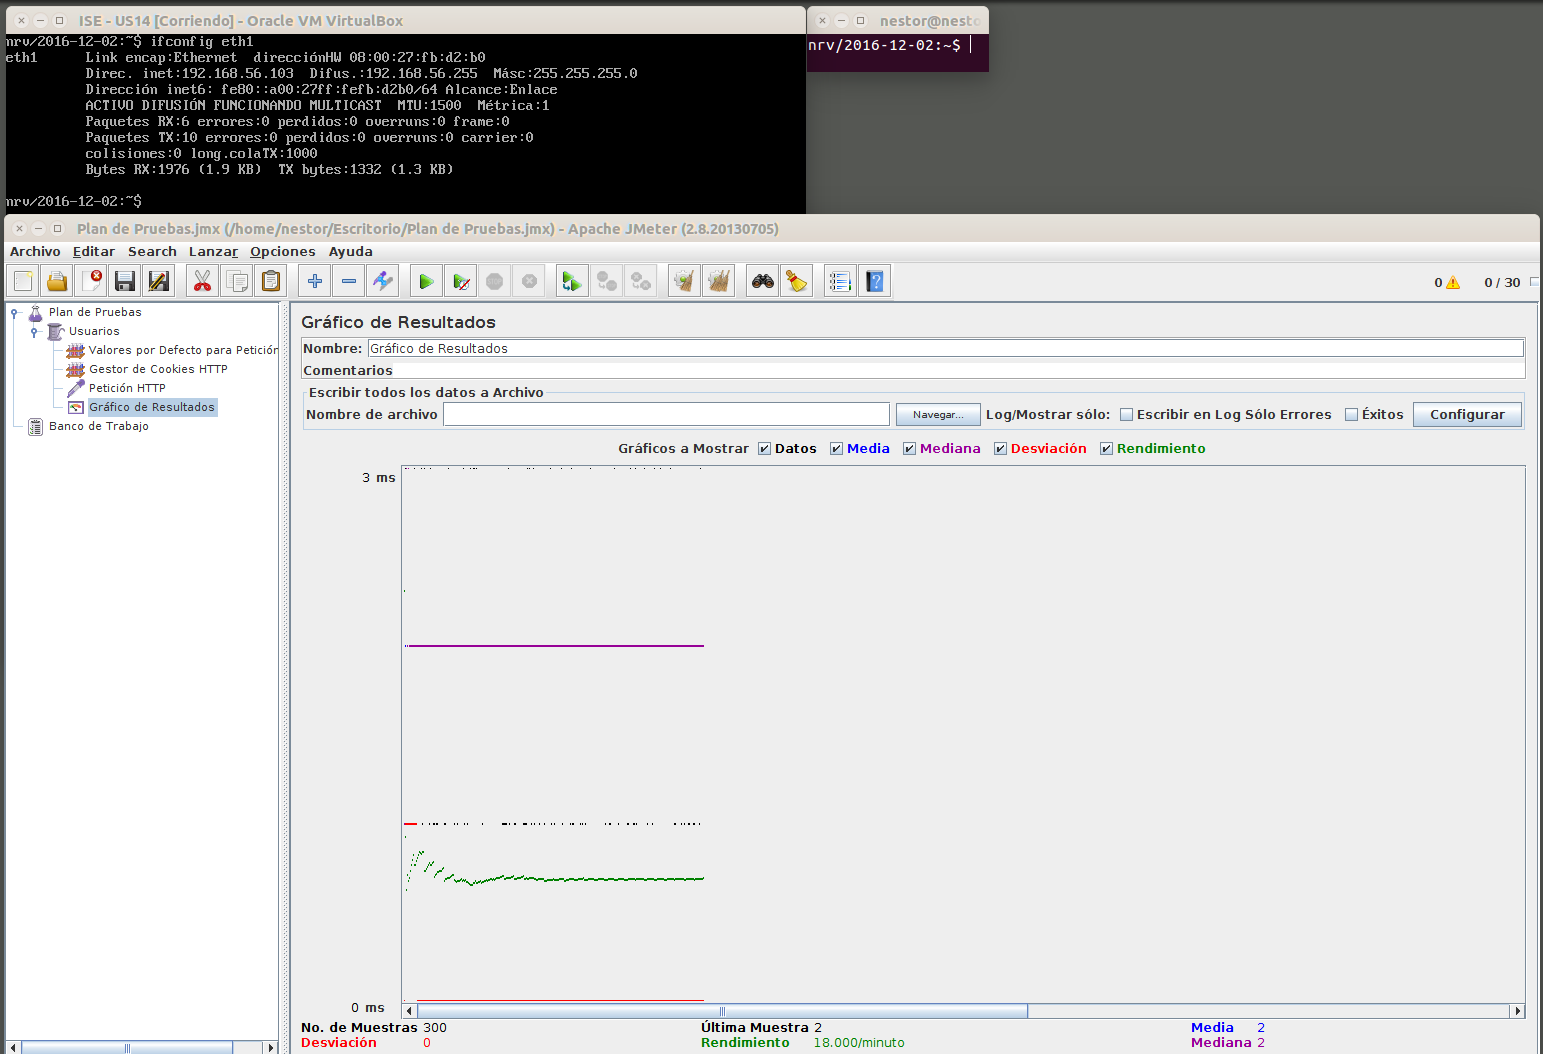
\includegraphics[width=\linewidth]{./Imagenes/4-resultado.png}
		\vspace{-0.5cm}
		\caption[Resultado de \textit{JMeter}.]{Resultado de \textit{JMeter}.}
		\label{4-resultado}
	\end{figure}
	
	%%%%%%%%%%%%%%%%%%%%%%%%%%%%%%%%%%%%%%%%%%%%%%%%%%%%
	%%%%%%%%%%%%%%%%%%%% Cuestión 5 %%%%%%%%%%%%%%%%%%%%
	%%%%%%%%%%%%%%%%%%%%%%%%%%%%%%%%%%%%%%%%%%%%%%%%%%%%
	\section[Cuestión 5: Programe un benchmark usando el lenguaje que desee. El	benchmark debe incluir: 1) Objetivo del benchmark. 2) Métricas (unidades, variables, puntuaciones, etc.). 3) Instrucciones para su uso. 4) Ejemplo de uso analizando los resultados.]{Cuestión 5: Programe un benchmark usando el lenguaje que desee. El	benchmark debe incluir: 1) Objetivo del benchmark. 2) Métricas (unidades, variables, puntuaciones, etc.). 3) Instrucciones para su uso. 4) Ejemplo de uso analizando los resultados.}
	
	\begin{enumerate}
		\item El objetivo del benchmark es conseguir un tiempo de ejecución para una tarea predeterminada para poder comparar distintas CPU. El benchmark consiste en la multiplicación de dos matrices y la escritura del resultado en una tercera matriz. La multiplicación se ha realizado de dos maneras: de forma secuencial y usando paralelización.
		
		\item La ejecución del benchmark devuelve dos tiempos, uno para la ejecución secuencial y otro para la ejecución en paralelo. El tiempo de la ejecución secuencial, nos indica el tiempo empleado en la multiplicación usando una hebra mientras que el tiempo de ejecución usando paralelización nos indica el tiempo empleado en la multiplicación usando todas las hebras que permita la arquitectura de la máquina. A parte de los tiempos, nos devuelve una puntuación, ya que tradicionalmente los benchmarks suelen darte una puntuación para tener una referencia más visual. Dicha puntuación se calcula como \textit{10000/tiempo}. Una mayor puntuación indica un mejor resultado.
		
		\item Para usar este benchmark lo compilamos ejecutando \textit{g++ -fopenmp benchmark.cpp -o benchmark}. Lo ejecutamos mediante el comando \textit{./benchmark}. A continuación nos pide el número de veces que se va a calcular la multiplicación de las matrices, para así luego poder calcular el tiempo medio de dichas ejecuciones.
		
		\item El resultado de la ejecución del benchmark en mi máquina se puede ver en la figura \ref{5-benchmark}. Podemos ver que en mi caso, el tiempo medio de ejecución para una ejecución secuencial es de 4.96044, obteniendo así una puntuación de 2015.95. En el caso de la ejecución paralela, el tiempo medio de ejecución es de 2.43497, obteniendo así una puntuación de 4106.83.
	\end{enumerate}
	
	\begin{figure}[H]
		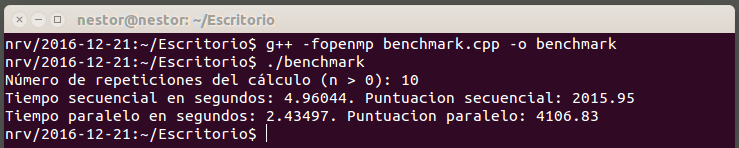
\includegraphics[width=\linewidth]{./Imagenes/5-benchmark.png}
		\vspace{-0.5cm}
		\caption[Resultado del benchmark.]{Resultado del benchmark.}
		\label{5-benchmark}
	\end{figure}
	
	El benchmark usado lo podemos ver a continuación \footnote{El benchmark \textit{``benchmark.cpp''} se encuentra dentro de la carpeta \textit{Archivos auxiliares}.}:
	\lstset{language=C++, breaklines=true, basicstyle=\footnotesize}
	\begin{lstlisting}[frame=single]
#include <iomanip>
#include <iostream>
#include <omp.h>
#include <vector>

using namespace std;

double t1secuencial, t2secuencial, t1paralelo, t2paralelo, t1, t2;
double M1[1000][1000], M2[1000][1000], M3[1000][1000];

double media(const vector<double> &elementos){
	double suma=0;
	for(int i=0; i<elementos.size(); i++)
		suma+=elementos[i];
	return suma/elementos.size();
}

void producto_secuencial(){
	int i, j, k;
	t1secuencial = omp_get_wtime();
	for (i=0; i<1000; i++){
		for(j=0; j<1000; j++){
			for (k=0; k<1000; k++){
				M1[i][j] = M1[i][j] + (M2[i][k]*M3[k][j]);
			}
		}
	}
	t2secuencial=omp_get_wtime();
}

void producto_paralelo(){
	int i, j, k;
	#pragma omp parallel shared(M1,M2,M3) private(i,j,k)
	{
		//Medida de tiempo
		#pragma omp single
		{
			t1paralelo = omp_get_wtime();
		}
		#pragma omp for schedule (runtime)
		for(i=0;i<1000; i++){
			for(j=0;j<1000; j++){
				for(k=0;k<1000; k++){
					M1[i][j] = M1[i][j] + M2[i][k] * M3[k][j];
				}
			}
		}
		//Medida de tiempo
		#pragma omp single
		{
			t2paralelo = omp_get_wtime();
		}
	}
}

int main(int argc, char *argv[]){
	vector<double> vtsecuencia, vtparalelo;
	int i, j, iteraciones = 0;
	cout << "Número de repeticiones del cálculo (n > 0): ";
	cin >> iteraciones;

	for (i=0; i<1000; i++){
		for (j=0; j<1000; j++){
			M1[i][j] = 0;
			M2[i][j] = 2;
			M3[i][j] = 2;
		}
	}

	for(int i=0; i<iteraciones; i++){
		producto_secuencial();
		vtsecuencia.push_back(t2secuencial - t1secuencial);
	}

	for (i=0; i<1000; i++){
		for (j=0; j<1000; j++){
			M1[i][j] = 0;
			M2[i][j] = 2;
			M3[i][j] = 2;
		}
	}

	for(int i=0; i<iteraciones; i++){
		producto_paralelo();
		vtparalelo.push_back(t2paralelo - t1paralelo);
	}

	t1 = media(vtsecuencia);
	t2 = media(vtparalelo);
	
	//Para evitar que el compilador suprima codigo:
	M1[0][0]++; M1[0][0]--;
	M2[0][0]++; M2[0][0]--;
	M3[0][0]++; M3[0][0]--;

	cout << "Tiempo secuencial en segundos: " << t1 << ". Puntuacion secuencial: " << 10000/t1 << endl;
	cout << "Tiempo paralelo en segundos: " << t2 << ". Puntuacion paralelo: " << 10000/t2 << endl;

	return 0;
}
	\end{lstlisting}
	
	%%%%%%%%%%%%%%%%%%%%%%%%%%%%%%%%%%%%%%%%%%%%%%%%%%%%
	%%%%%%%%%%%%%%%%%%%% Cuestión Opcional 1 %%%%%%%%%%%
	%%%%%%%%%%%%%%%%%%%%%%%%%%%%%%%%%%%%%%%%%%%%%%%%%%%%
	\section[Cuestión opcional 1: ¿Qué es Scala? Instale Gatling y pruebe los escenarios por defecto.]{Cuestión opcional 1: ¿Qué es Scala? Instale Gatling y pruebe los escenarios por defecto.}
	
	Para saber que es \textit{Scala} no hay nada mejor que verlo en la página oficial \cite{scala}. \textit{Scala} es un lenguaje de programación. \textit{Scala} es el acrónimo de \textit{``Scalable Language''}. Podemos usar \textit{Scala} para programación orientada a objetos o para una programación más funcional. Se ejecuta sobre la máquina virtual de Java. Las clases de \textit{Java} y \textit{Scala} pueden combinarse sin ningún problema. \\
	
	Como podemos ver en la página de \textit{Gatling} \cite{gatling}, \textit{Gatling} se basa en \textit{Scala}, así que primero tenemos que instalar \textit{Scala}, en mi caso en Ubuntu Server. Para ello ejecutamos \textit{sudo apt install scala}, como podemos ver en la figura \ref{O1-instalacion}. Una vez instalado, pasamos a instalar \textit{Gatling} siguiendo las instrucciones que podemos ver en la página oficial \cite{gatling_download}. Debemos descargar un fichero zip y luego extraerlo. Una vez extraído, dentro de la carpeta de \textit{Gatling} nos encontramos la carpeta \textit{bin} y dentro de ella el fichero \textit{gatling.sh}. Lo ejecutamos mediante el comando \textit{./gatling.sh} como podemos ver en la figura \ref{O1-1}. A continuación nos pedirá que escenario queremos usar como podemos ver en la figura \ref{O1-1}, yo he elegido el 0. A continuación comenzará la prueba. El resultado lo podemos ver en la figura \ref{O1-2}.
	
	\begin{figure}[H]
		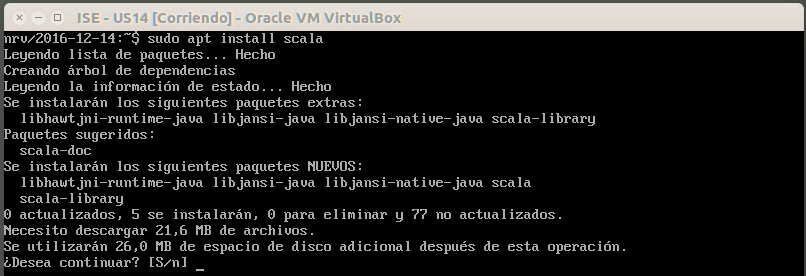
\includegraphics[width=\linewidth]{./Imagenes/O1-instalacion.png}
		\vspace{-0.5cm}
		\caption[Instalación de \textit{Scala}.]{Instalación de \textit{Scala}.}
		\label{O1-instalacion}
	\end{figure}
	
	\begin{figure}[H]
		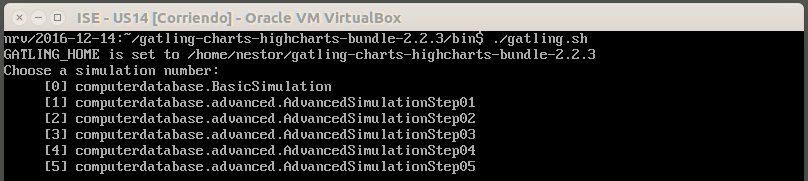
\includegraphics[width=\linewidth]{./Imagenes/O1-1.png}
		\vspace{-0.5cm}
		\caption[Ejecución de \textit{Gatling} y posibles escenarios.]{Ejecución de \textit{Gatling} y posibles escenarios.}
		\label{O1-1}
	\end{figure}
	
	\begin{figure}[H]
		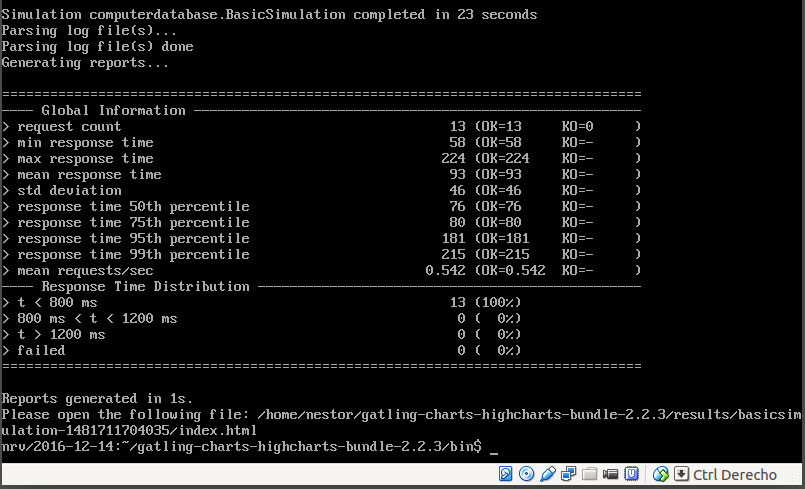
\includegraphics[width=\linewidth]{./Imagenes/O1-2.png}
		\vspace{-0.5cm}
		\caption[Resultado de la ejecución de \textit{Gatling}.]{Resultado de la ejecución de \textit{Gatling}.}
		\label{O1-2}
	\end{figure}
	
	Para poder ver los resultados de una mejor forma, copiamos el contenido de la carpeta \textit{/results/basicsimulation-1481711704035} a \textit{/var/www/html}, para poder acceder desde el navegador de mi máquina anfitriona. Para ello, desde la carpeta \textit{/results/basicsimulation-1481711704035} ejecutamos \textit{cp -r * /var/www/html}, como podemos ver en la figura \ref{O1-3}. A continuación, accedemos desde la máquina anfitriona. Para ello introducimos la dirección IP de nuestro servidor seguido de \textit{/index.html}. Como podemos ver en la figura \ref{O1-3} la dirección IP de mi servidor es \textit{192.168.56.103} (máquinas conectas en modo \textit{host-only}), así que debemos introducir \textit{192.168.56.103/index.html}. Podemos ver los resultados en la figura \ref{O1-4}. Como podemos ver, se han respondido todas las solicitudes de manera correcta y todas en menos de 800ms. 
	
	\begin{figure}[H]
		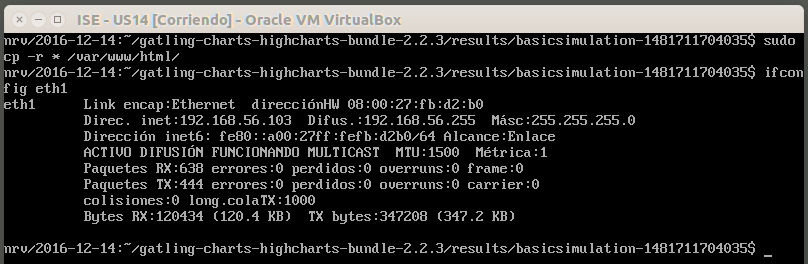
\includegraphics[width=\linewidth]{./Imagenes/O1-3.png}
		\vspace{-0.5cm}
		\caption[Copia de los resultados y dirección IP del servidor.]{Copia de los resultados y dirección IP del servidor.}
		\label{O1-3}
	\end{figure}
	
	\begin{figure}[H]
		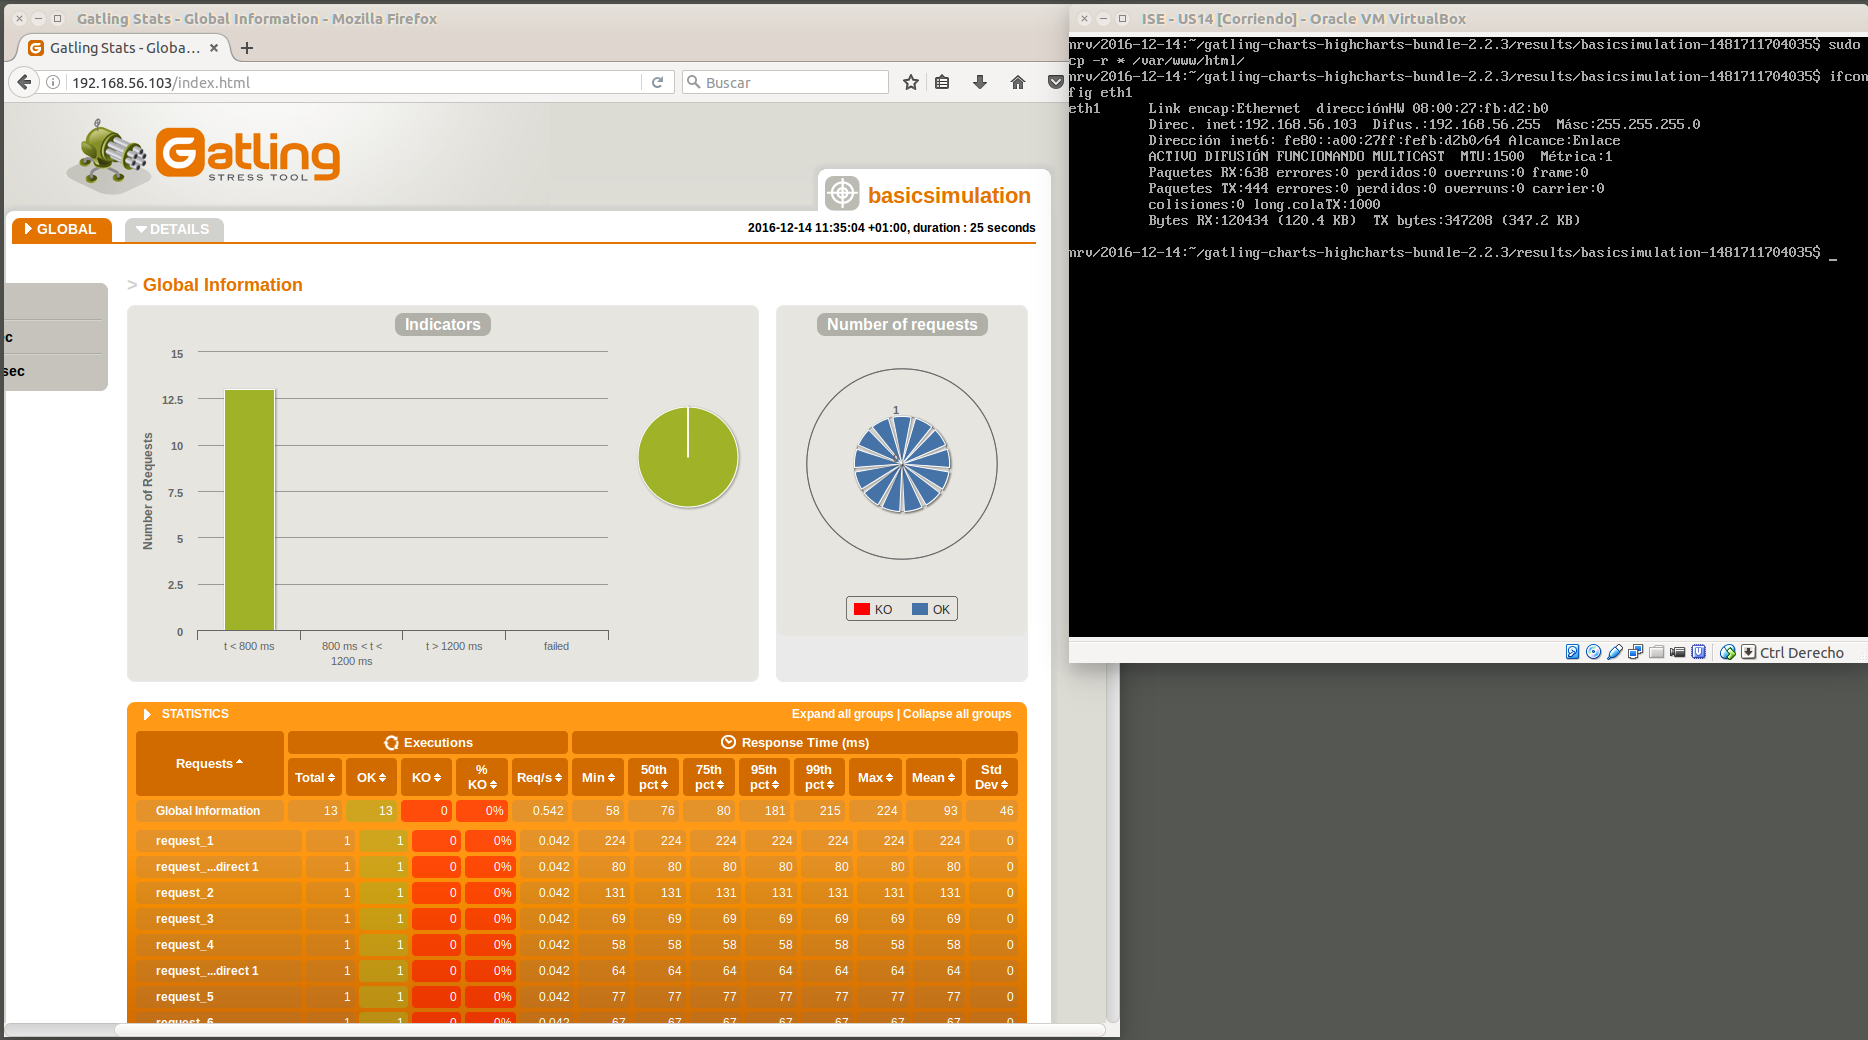
\includegraphics[width=\linewidth]{./Imagenes/O1-4.png}
		\vspace{-0.5cm}
		\caption[Resultado de \textit{Gatling} desde el navegador.]{Resultado de \textit{Gatling} desde el navegador.}
		\label{O1-4}
	\end{figure}
	
	\clearpage
	\bibliography{bibliografia}
	\bibliographystyle{ieeetr}
\end{document}